\documentclass{beamer}
\usepackage[T1]{fontenc}
\usepackage[utf8]{inputenc}

\usetheme{Madrid}
\usecolortheme{default}
\usepackage{amsmath,amssymb,amsfonts,amsthm}
\usepackage{txfonts}
\usepackage{tkz-euclide}
\usepackage{listings}
\usepackage{adjustbox}
\usepackage{array}
\usepackage{tabularx}
\usepackage{gvv}
\usepackage{lmodern}
\usepackage{gensymb}
\usepackage{circuitikz}
\usepackage{tikz}
\usepackage{graphicx}
\usepackage{capt-of}

\setbeamertemplate{page number in head/foot}[totalframenumber]

\usepackage{tcolorbox}
\tcbuselibrary{minted,breakable,xparse,skins}

\definecolor{bg}{gray}{0.95}
\DeclareTCBListing{mintedbox}{O{}m!O{}}{%
  breakable=true,
  listing engine=minted,
  listing only,
  minted language=#2,
  minted style=default,
  minted options={%
    linenos,
    gobble=0,
    breaklines=true,
    breakafter=,,
    fontsize=\small,
    numbersep=8pt,
    #1},
  boxsep=0pt,
  left skip=0pt,
  right skip=0pt,
  left=25pt,
  right=0pt,
  top=3pt,
  bottom=3pt,
  arc=5pt,
  leftrule=0pt,
  rightrule=0pt,
  bottomrule=2pt,
  toprule=2pt,
  colback=bg,
  colframe=orange!70,
  enhanced,
  overlay={%
    \begin{tcbclipinterior}
    \fill[orange!20!white] (frame.south west) rectangle ([xshift=20pt]frame.north west);
    \end{tcbclipinterior}},
  #3,
}
\lstset{
    language=C,
    basicstyle=\ttfamily\small,
    keywordstyle=\color{blue},
    stringstyle=\color{orange},
    commentstyle=\color{green!60!black},
    numbers=left,
    numberstyle=\tiny\color{gray},
    breaklines=true,
    showstringspaces=false,
}

\title{4.2.13}
\subtitle{Direction and normal vector}
\author{EE25BTECH11010 - Arsh Dhoke}
\date{}
\begin{document}


\begin{frame}
  \titlepage
\end{frame}


\begin{frame}{Question}
\textbf{Question:}\\
 Find the direction and normal vector for the line y = x.
\end{frame}

\begin{frame}{Solution}
The line can be written as: 
\begin{align}
x - y = 0
\end{align}

Let
\begin{align}
\vec{x} = \myvec{x \\ y}, \quad
\vec{n^T} = \myvec{1 & -1}, \quad
c = 0
\end{align}

Then:
\begin{align}
\vec{n^T} \vec{x} = c
\end{align}

Where \(\vec{n}\) is the normal vector of the given line.
\end{frame}

\begin{frame}{Direction Vector}
The direction vector of the line is:
\begin{align}
\vec{m} = \myvec{1 \\ 1}
\end{align}

If the direction vector is given by
\begin{align}
\vec{m} = \myvec{1 \\ m}
\end{align}
then the normal vector can be written as
\begin{align}
\vec{n} = \myvec{-m \\ 1}
\end{align}

We can prove this using
\begin{align}
\vec{n^T}\vec{m} = 0
\end{align}


\end{frame}

\begin{frame}{Final Vectors}
\begin{align}
\myvec{1 & -1}\myvec{1 \\ 1} = 0
\end{align}
The normal vector of the line is 
$
\vec{n} = \myvec{1 \\ -1}
$

The direction vector of the line is 
$
\vec{m} = \myvec{1 \\ 1}
$
\end{frame}

\begin{frame}{Graph}
\begin{figure}[ht!]
\centering
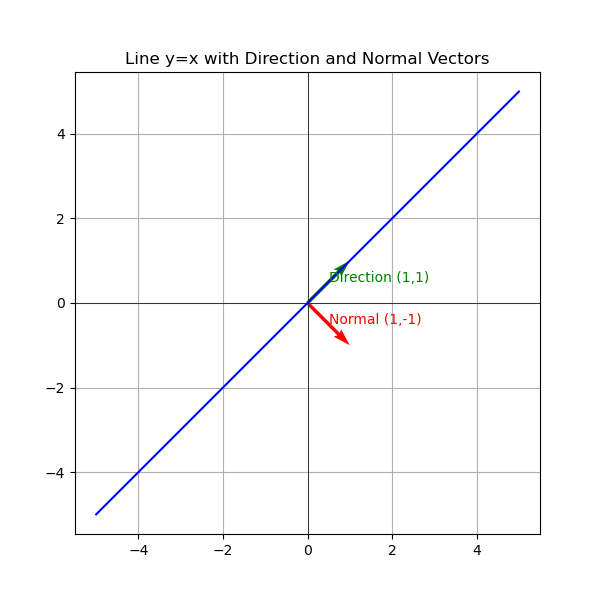
\includegraphics[height=0.6\textheight, keepaspectratio]{figs/q6.png}
\caption{Graph of the line with direction and normal vectors}
\end{figure}
\end{frame}

\begin{frame}[fragile]
    \frametitle{C Code}
\begin{lstlisting}
typedef struct {
    double nx;
    double ny;
    double dx;
    double dy;
} LineVectors;

LineVectors find_vectors(double a, double b, double c) {
    LineVectors result;
    result.nx = a;
    result.ny = b;
    result.dx = -b;
    result.dy = a;
    return result;
}

\end{lstlisting}
\end{frame}

\begin{frame}[fragile]
    \frametitle{Python Code}
\begin{lstlisting}
import numpy as np
import matplotlib.pyplot as plt

# Define the line y = x
x_vals = np.linspace(-5, 5, 100)
y_vals = x_vals

# Normal and direction vectors
normal_vec = np.array([1, -1])
direction_vec = np.array([1, 1])

# Choose a point on the line (origin for simplicity)
point = np.array([0, 0])

# Create the plot
plt.figure(figsize=(6,6))
plt.axhline(0, color='black', linewidth=0.5)  # x-axis
plt.axvline(0, color='black', linewidth=0.5)  # y-axis
\end{lstlisting}
\end{frame}

\begin{frame}[fragile]
    \frametitle{Python Code}
\begin{lstlisting}
# Plot the line
plt.plot(x_vals, y_vals, 'b', label='y = x')

# Plot the direction vector (along the line)
plt.quiver(point[0], point[1],
           direction_vec[0], direction_vec[1],
           angles='xy', scale_units='xy', scale=1, color='green')
plt.text(direction_vec[0]/2, direction_vec[1]/2, 'Direction (1,1)', color='green')

# Plot the normal vector (perpendicular to the line)
plt.quiver(point[0], point[1],
           normal_vec[0], normal_vec[1],
           angles='xy', scale_units='xy', scale=1, color='red')
plt.text(normal_vec[0]/2, normal_vec[1]/2, 'Normal (1,-1)', color='red')
\end{lstlisting}
\end{frame}

\begin{frame}[fragile]
    \frametitle{Python Code}
\begin{lstlisting}
# Formatting
plt.xlim(-5,5)
plt.ylim(-5,5)
plt.axis('equal')
plt.grid(True)
plt.title('Line y=x with Direction and Normal Vectors')
plt.savefig("/home/arsh-dhoke/ee1030-2025/ee25btech11010/matgeo/4.2.13/figs/q6.png")
plt.show()

\end{lstlisting}
\end{frame}

\begin{frame}[fragile]
    \frametitle{Python+ C Code}
\begin{lstlisting}
import ctypes
import matplotlib.pyplot as plt
import numpy as np

# Load shared library
lib = ctypes.CDLL('./code.so')  

# Define the struct in Python
class LineVectors(ctypes.Structure):
    _fields_ = [
        ('nx', ctypes.c_double),
        ('ny', ctypes.c_double),
        ('dx', ctypes.c_double),
        ('dy', ctypes.c_double)
    ]

# Function signature
\end{lstlisting}
\end{frame}

\begin{frame}[fragile]
    \frametitle{Python+ C Code}
\begin{lstlisting}
lib.find_vectors.restype = LineVectors
lib.find_vectors.argtypes = [ctypes.c_double, ctypes.c_double, ctypes.c_double]

# Call the function for y = x -> x - y = 0 -> a=1, b=-1, c=0
v = lib.find_vectors(1.0, -1.0, 0.0)

# Print results
print("Normal vector:", (v.nx, v.ny))
print("Direction vector:", (v.dx, v.dy))

# Plotting the line and direction vector
# Line equation: a*x + b*y + c = 0 -> y = (-a*x - c)/b
a, b, c = 1.0, -1.0, 0.0
x_vals = np.linspace(-5, 5, 100)
y_vals = (-a * x_vals - c) / b

plt.figure(figsize=(6,6))
\end{lstlisting}
\end{frame} 

\begin{frame}[fragile]
    \frametitle{Python+ C Code}
\begin{lstlisting}
plt.plot(x_vals, y_vals, label='Line y = x', color='blue')

# Plot direction vector as an arrow from origin
plt.quiver(0, 0, v.dx, v.dy, angles='xy', scale_units='xy', scale=1, color='red', label='Direction vector')

# Plot normal vector as arrow from origin
plt.quiver(0, 0, v.nx, v.ny, angles='xy', scale_units='xy', scale=1, color='green', label='Normal vector')

plt.xlim(-6,6)
plt.ylim(-6,6)
plt.gca().set_aspect('equal', adjustable='box')
plt.grid(True)
plt.legend()
plt.title("Line y = x with Normal and Direction Vectors")
plt.savefig("/home/arsh-dhoke/ee1030-2025/ee25btech11010/matgeo/4.2.13/figs/q6.png")
plt.show()

\end{lstlisting}
\end{frame}

\end{document}